\PassOptionsToPackage{unicode=true}{hyperref} % options for packages loaded elsewhere
\PassOptionsToPackage{hyphens}{url}
%
\documentclass[]{article}
\usepackage{lmodern}
\usepackage{setspace}
\setstretch{2}
\usepackage{amssymb,amsmath}
\usepackage{ifxetex,ifluatex}
\usepackage{fixltx2e} % provides \textsubscript
\ifnum 0\ifxetex 1\fi\ifluatex 1\fi=0 % if pdftex
  \usepackage[T1]{fontenc}
  \usepackage[utf8]{inputenc}
  \usepackage{textcomp} % provides euro and other symbols
\else % if luatex or xelatex
  \usepackage{unicode-math}
  \defaultfontfeatures{Ligatures=TeX,Scale=MatchLowercase}
\fi
% use upquote if available, for straight quotes in verbatim environments
\IfFileExists{upquote.sty}{\usepackage{upquote}}{}
% use microtype if available
\IfFileExists{microtype.sty}{%
\usepackage[]{microtype}
\UseMicrotypeSet[protrusion]{basicmath} % disable protrusion for tt fonts
}{}
\IfFileExists{parskip.sty}{%
\usepackage{parskip}
}{% else
\setlength{\parindent}{0pt}
\setlength{\parskip}{6pt plus 2pt minus 1pt}
}
\usepackage{hyperref}
\hypersetup{
            pdftitle={Physcraper: a python package for continual update of evolutionary estimates using the Open Tree of Life},
            pdfborder={0 0 0},
            breaklinks=true}
\urlstyle{same}  % don't use monospace font for urls
\usepackage[margin = 1in]{geometry}
\usepackage{longtable,booktabs}
% Fix footnotes in tables (requires footnote package)
\IfFileExists{footnote.sty}{\usepackage{footnote}\makesavenoteenv{longtable}}{}
\usepackage{graphicx,grffile}
\makeatletter
\def\maxwidth{\ifdim\Gin@nat@width>\linewidth\linewidth\else\Gin@nat@width\fi}
\def\maxheight{\ifdim\Gin@nat@height>\textheight\textheight\else\Gin@nat@height\fi}
\makeatother
% Scale images if necessary, so that they will not overflow the page
% margins by default, and it is still possible to overwrite the defaults
% using explicit options in \includegraphics[width, height, ...]{}
\setkeys{Gin}{width=\maxwidth,height=\maxheight,keepaspectratio}
\setlength{\emergencystretch}{3em}  % prevent overfull lines
\providecommand{\tightlist}{%
  \setlength{\itemsep}{0pt}\setlength{\parskip}{0pt}}
\setcounter{secnumdepth}{5}
% Redefines (sub)paragraphs to behave more like sections
\ifx\paragraph\undefined\else
\let\oldparagraph\paragraph
\renewcommand{\paragraph}[1]{\oldparagraph{#1}\mbox{}}
\fi
\ifx\subparagraph\undefined\else
\let\oldsubparagraph\subparagraph
\renewcommand{\subparagraph}[1]{\oldsubparagraph{#1}\mbox{}}
\fi

% set default figure placement to htbp
\makeatletter
\def\fps@figure{htbp}
\makeatother

\usepackage{color}
\usepackage{hyperref}
\usepackage{caption}
\usepackage{blindtext}
\usepackage{url}
\usepackage[left]{lineno}
\linenumbers

\title{Physcraper: a python package for continual update of evolutionary estimates using the Open Tree of Life}
\author{}
\date{\vspace{-2.5em}}

\begin{document}
\maketitle

\textbf{1. Luna L. Sanchez Reyes}

School of Natural Sciences, University of California, Merced

email: \href{mailto:sanchez.reyes.luna@gmail.com}{\nolinkurl{sanchez.reyes.luna@gmail.com}}

\textbf{2. Martha Kandziora}

School of Natural Sciences, University of California, Merced

Department of Botany, Faculty of Science, Charles University, Prague, Czech Republic

email: \href{mailto:kandziom@natur.cuni.cz}{\nolinkurl{kandziom@natur.cuni.cz}}

\textbf{3. Emily Jane McTavish}

School of Natural Sciences, University of California, Merced

email: \href{mailto:ejmctavish@gmail.com}{\nolinkurl{ejmctavish@gmail.com}}

\textbf{Correspondence address}: Science and Engineering Building 1, University of California, Merced, 5200 N. Lake Rd, Merced CA 95343

\textbf{Correspondence email}: \href{mailto:sanchez.reyes.luna@gmail.com}{\nolinkurl{sanchez.reyes.luna@gmail.com}}, \href{mailto:ejmctavish@gmail.com}{\nolinkurl{ejmctavish@gmail.com}}

\textbf{Running title}: Updating gene trees with the Open Tree of Life

\textbf{Word count}: 2849

\textbf{Manuscript prepared for submission to Methods in Ecology and Evolution}

\textbf{Article type}: Application

\newpage

\begingroup\Large

\textbf{Abstract}
\endgroup

\begin{enumerate}
\def\labelenumi{\arabic{enumi}.}
\item
  Phylogenies are a key part of research in many areas of biology. Tools that automate
  some parts of the process of phylogenetic reconstruction, mainly molecular character matrix assembly,
  have been developed for the advantage of both specialists in the field of phylogenetics and nonspecialists.
  However, interpretation of results, comparison with previously available phylogenetic
  hypotheses, and choice of one phylogeny for downstream analyses and discussion still impose difficulties
  to one that is not a specialist either on phylogenetic methods or on a particular group of study.
\item
  Physcraper is a command-line Python program that automates the update of published
  phylogenies by adding public DNA sequences to underlying alignments of previously published phylogenies. It also provides a framework for straightforward comparison of published phylogenies with their updated versions, by leveraging upon tools from the Open Tree of Life project to link taxonomic information across databases.
\item
  Physcraper can be used by the nonspecialist, as a tool to generate phylogenetic
  hypotheses based on publicly available expert phylogenetic knowledge.
  Phylogeneticists and taxonomic group specialists will find it useful as a tool to facilitate molecular dataset gathering and comparison
  of alternative phylogenetic hypotheses (topologies).
\item
  The Physcraper workflow demonstrates the benefits of doing open science for phylogenetics, encouraging more researchers to strive for better sharing practices. Physcraper can be used with any OS and is released under an open-source license. Detailed instructions for installation and
  use are available at \href{https://physcraper.readthedocs.io}{https://physcraper.readthedocs}.
\end{enumerate}

\textbf{Keywords}: gene tree, interoperability, open science, open tree of life, phylogeny, public database, python, reproducibility, taxonomy, updated alignment

\newpage

\hypertarget{introduction}{%
\section{Introduction}\label{introduction}}

Phylogenies capture the shared history of living and extinct organisms and provide key evolutionary context for all our biological observations.
Public biological databases constitute an amazing resource for evolutionary studies, but a large portion of molecular data publicly available has never been incorporated into any phylogenetic estimate. Extending existing phylogenies with new DNA sequence data, geographical location, and other metadata in a reproducible and continuous manner is possible by automating connections between biological databases. Here, we introduce Physcraper, a tool to build upon molecular data that taxon specialists have assessed and deemed appropriate for a specific phylogenetic scope, by using sequence data from public biological databases to update a starting tree and single locus alignments.

Automatic integration of data in a phylogenetic context is challenged by the prevalence of taxonomic idiosyncrasies across biological databases. Taxonomic name standardization represents a step toward tackling this issue, but requires a unified system. The Open Tree of Life project (OpenTree)
has constructed a comprehensive tree of life by synthesizing published phylogenies along with taxonomic data. OpenTree's ``synthetic'' tree comprises 2.3 million tips, of which around 90,000 are supported by phylogenetic estimates - the remaining 1.4 million taxa are placed in the tree based on taxonomy. To achieve this, OpenTree unifies taxonomy from various databases (Rees \& Cranston \protect\hyperlink{ref-rees2017automated}{2017}), including the USA National Center for Biodiversity Information (NCBI) molecular database GenBank (Benson \emph{et al.} \protect\hyperlink{ref-benson2000genbank}{2000}; Wheeler \emph{et al.} \protect\hyperlink{ref-wheeler2000database}{2000}), the Global Biodiversity Information Facility (GBIF; Secretariat \protect\hyperlink{ref-secretariat2017gbif}{2017}), the World Register of Marine Species (WoRMS), and other resources. The OpenTree unified taxonomy represents a key resource for connecting data from virtually any biological database to phylogenetic data that has been standardized to OpenTree's unified taxonomy.

Another challenge to incorporating molecular data from public databases to update phylogenetic knowledge is assembling high-quality homology hypotheses.
Species tree reconstructions from multiple single locus data sets taking into account the multispecies coalescent model are considered the gold standard for inferring species relationships (Song \emph{et al.} \protect\hyperlink{ref-song2012resolving}{2012}).
Genomics has, and will continue to, revolutionize phylogenetic inference.
Yet, different research questions call for different genomic sequencing approaches (e.g., whole genomes, microsatellites, ultra-conserved elements), which produce largely non-overlapping genomic data sets across taxa, creating challenges in wide scale phylogenetic reconstruction.
While phylogenomics ameliorates the problem of non-overlapping genomic data sets by focusing on targeted capture of informative characters from independent and single-copy genetic markers (Jones \& Good \protect\hyperlink{ref-jones2016targeted}{2016}; Andermann \emph{et al.} \protect\hyperlink{ref-andermann2020guide}{2020}), decades of single locus sequencing have generated massive amounts of homologous DNA data sets that can be used for phylogenetic reconstruction at many scales.
Even in phylogenomic reconstructions, thoughtfully curated markers and alignments can improve phylogenetic reconstructions (Fragoso-Martínez \emph{et al.} \protect\hyperlink{ref-fragoso2017pilot}{2017}).

More than a decade ago, GenBank release number 159 (April 15, 2007) already hosted 72 million DNA sequences. These sequences were gauged to have the potential to resolve phylogenetic relationships of most (98.05\%) of the almost 241, 000 distinct taxa in the NCBI taxonomy at the time (Sanderson \emph{et al.} \protect\hyperlink{ref-sanderson2008phylota}{2008}). Assembling a DNA alignment from such a massive database can be done ``by hand'', but it requires huge amounts of time and it is mostly a non-reproducible approach. Computational pipelines that make DNA sequence search faster and more efficient, as well as more reproducible, have been applied to study evolutionary relationships among a variety of organisms (e.g., Smith \emph{et al.} \protect\hyperlink{ref-smith2009mega}{2009}; Izquierdo-Carrasco \emph{et al.} \protect\hyperlink{ref-izquierdo2014pumper}{2014}; Antonelli \emph{et al.} \protect\hyperlink{ref-antonelli2017toward}{2017}).

A way to incorporate the benefits from massive amounts of newly released molecular data and fine-grained curation from human experts, is to rely on manually curated homology hypotheses as ``jump-start'' alignments (Morrison \protect\hyperlink{ref-morrison2006multiple}{2006}). The TreeBASE database (Piel \emph{et al.} \protect\hyperlink{ref-piel2009treebase}{2009}) hosts about 8, 200 alignments, providing information on evolutionary relationships of around 100, 000 distinct taxa \href{https://www.treebase.org/treebase-web/home.html\#:~:text=TreeBASE\%20is\%20produced\%20and\%20governed,mapped\%20to\%20104\%2C593\%20distinct\%20taxa.}{(see TreeBASE's website about)}, representing a public source of valuable expert knowledge. Linking published alignments with molecular data that has not yet been included in any public phylogenetic estimate, has the potential to accelerate the enrichment and updating of phylogenetic relationships in many regions of the tree of life.

Physcraper relies on programmatic access protocols (API's) to automatically link molecular data from GenBank to alignments from TreeBASE and phylogenies from OpenTree's Phylesystem, to continually update and enrich phylogenetic knowledge based on expertly-curated homology hypotheses. Physcraper also provides new types of access to various OpenTree tools for comparison of existing phylogenetic hypotheses with newly generated ones.
Physcraper is coded as a Python pipeline that focuses on data interoperability, by using the standardized taxonomy as a way to link taxon data from different databases. This integration also allows users to rapidly place new data from a diverse range of biological databases in an evolutionary context, opening the possibility for a variety of comparative downstream analyses.

\hypertarget{the-physcraper-framework}{%
\section{The Physcraper framework}\label{the-physcraper-framework}}

\begin{figure}

{\centering 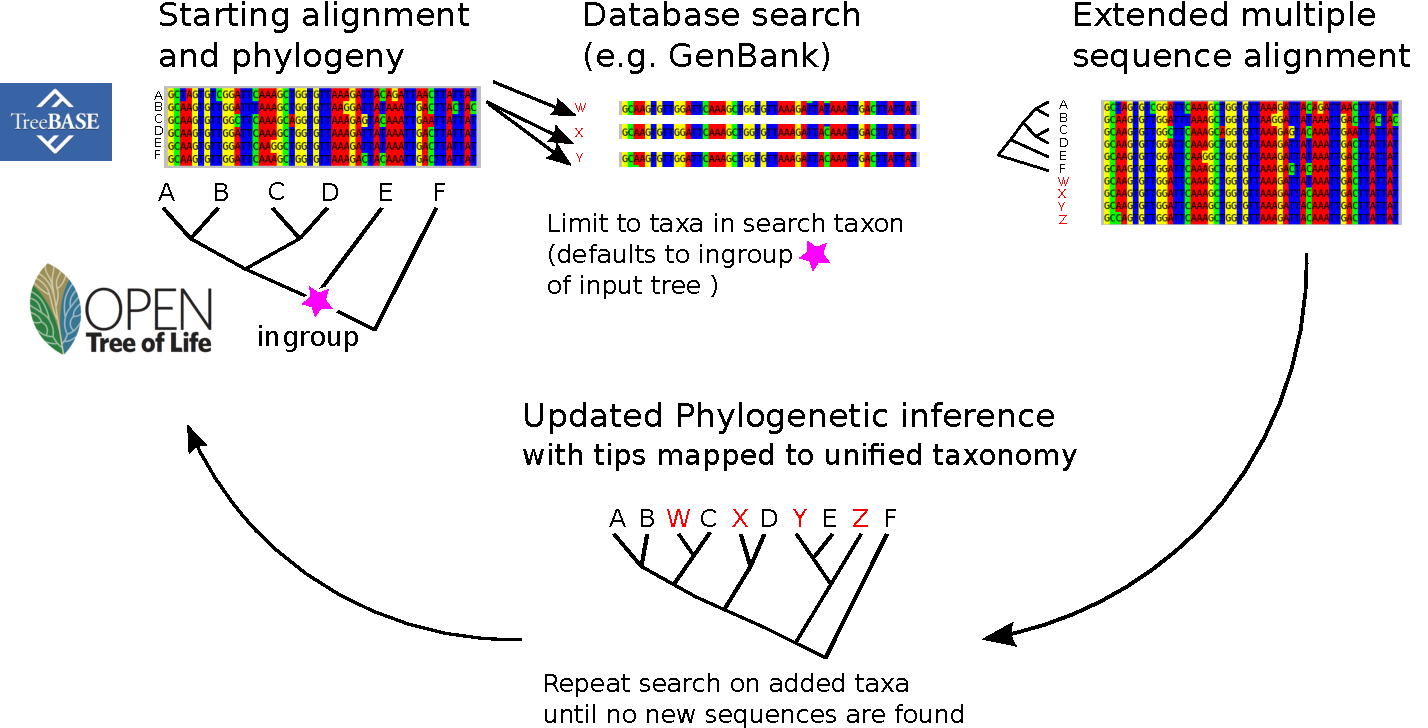
\includegraphics[width=0.85\linewidth]{docs/figs/schematic} 

}

\caption{The Physcraper framework consists of 4 steps (see text). The software is fully described on its documentation website at physcraper.readthedocs.io, along with installation instructions, function usage descriptions, examples and tutorials.}\label{fig:framework}
\end{figure}

The general Physcraper framework is depicted in Figure \ref{fig:framework}. It consists of 4 steps: 1) identifying and processing a phylogenetic tree to update its underlying alignment; 2) performing a constrained BLAST search of DNA sequences in the original alignment on the GenBank database, and filtering of new sequences; 3) profile-aligning filtered new sequences to the original alignment; 4) performing a phylogenetic analysis and comparing the updated tree to previous phylogenetic estimates within the focus group.

\hypertarget{the-inputs-a-tree-and-an-alignment}{%
\subsection{The inputs: a tree and an alignment}\label{the-inputs-a-tree-and-an-alignment}}

Taxon names in the input tree must be standardized or ``mapped'' to the unified OpenTree taxonomy (Rees \& Cranston \protect\hyperlink{ref-rees2017automated}{2017}) using OpenTree's bulk Taxonomic Name Resolution Service \href{https://tree.opentreeoflife.org/curator/tnrs/}{TNRS} tool. Users can upload their own tree, or choose from among the 2, 950 mapped trees stored in OpenTree's \href{https://github.com/opentreeoflife/phylesystem}{Phylesystem} that also have alignments avilable on TreeBASE (Piel \emph{et al.} \protect\hyperlink{ref-piel2009treebase}{2009}; Vos \emph{et al.} \protect\hyperlink{ref-vos2012nexml}{2012}).

The input alignment should be a single locus alignment that was used in part or in whole, to generate the input tree. If the alignment associated to the input tree is stred in TreeBASE, Physcraper retrieves it automatically. Alignments stored in any other repository, or constituting personal data have to be downloaded by the user.

Physcraper processes the input tree to match taxa found in the alignment, and verifies that all taxon names on the tips of the tree are in the DNA character matrix and vice versa. Technically, just one taxon name and its corresponding sequence in the alignment are needed to continue the algorithm.

\hypertarget{dna-sequence-search-and-filtering}{%
\subsection{DNA sequence search and filtering}\label{dna-sequence-search-and-filtering}}

The DNA sequence search is performed with the Basic Local Alignment Search Tool, BLAST (Altschul \emph{et al.} \protect\hyperlink{ref-altschul1990basic}{1990}), either on the GenBank remote database or in a GenBank local database set up by the user. It is constrained to a taxonomic group in the NCBI taxonomy, defined as the ``search taxon''. Users can arbitrarily define a search taxon that is either a more or a less inclusive
clade relative to the ingroup of the input tree.
Otherwise, the search taxon is automatically identified using the OpenTree \href{https://github.com/OpenTreeOfLife/germinator/wiki/Taxonomy-API-v3\#mrca}{API} (Rees \& Cranston \protect\hyperlink{ref-rees2017automated}{2017}), as the Most Recent Common Ancestral Taxon (MRCAT) of the ingroup taxa in the input tree, i.e., the MRCA that is also a named clade in the NCBI taxonomy (Fig. \ref{fig:framework}).
The MRCAT can be different from the phylogenetic MRCA when the latter is an unnamed clade in the synthetic tree.

BLAST command line tools \texttt{blastn} function (Camacho \emph{et al.} \protect\hyperlink{ref-camacho2009blast}{2009}) is used for local database sequence searches.
For remote database searches, we modified the BioPython (Cock \emph{et al.} \protect\hyperlink{ref-cock2009biopython}{2009}) BLAST function from the \href{https://biopython.org/DIST/docs/api/Bio.Blast.NCBIWWW-module.html}{NCBIWWW module} to accept an alternative BLAST address (URL). This is useful when a user lacks access to the computer capacity needed to setup a local database, but has access to an institutional server.
Each sequence in the alignment is BLASTed once against all DNA sequences in GenBank within the search taxon. GenBank sequences with match scores smaller than the e-value cutoff (default to 0.00001) are downloaded into a local library.

Downlodaded sequences are not further considered in the analysis if they fall outside a min and max length threshold, defined as the proportion of the average length without gaps of all sequences in the input alignment (default values of 80\% and 120\%, respectively); or if they are either identical to or shorter than an existing sequence in the input alignment and they represent the same taxon in the OTT taxonomy or the NCBI taxonomy.
If there are several sequences per taxon, an arbitrary number of 5 (can be modified by the user) sequences per taxon are chosen at random.

Reverse, complement, and reverse-complement sequences are identified and translated using BioPython internal functions (Cock \emph{et al.} \protect\hyperlink{ref-cock2009biopython}{2009}).
Iterative cycles of BLAST searches can be performed, by blasting the new sequences until no new ones are found. By default only one BLAST search cycle is performed in which only sequences in the input alignment are blasted.

\hypertarget{new-dna-sequence-alignment}{%
\subsection{New DNA sequence alignment}\label{new-dna-sequence-alignment}}

By default, Physcraper uses MUSCLE (Edgar \protect\hyperlink{ref-edgar2004muscle}{2004}) to perform DNA sequence alignments in a two step process. First, all new sequences are aligned using the default MUSCLE options.

Second, a MUSCLE profile alignment is performed, in which the original alignment is used as a template to align the new sequences. This ensures that the final alignment
follows the homology criteria established by the original alignment.
The final alignment is not further processed by Physcraper. It is recommended that the alignment is checked by the user, by eye followed by manual refinement, or using a tool for automatic alignment processing (e.g., GBlocks; Castresana \protect\hyperlink{ref-castresana2000selection}{2000}).
Users may also use Physcraper to only gather new GenBank sequences, to then apply their own preferred alignment and phylogenetic inference methods.

\hypertarget{tree-reconstruction-and-comparison}{%
\subsection{Tree reconstruction and comparison}\label{tree-reconstruction-and-comparison}}

A Maximum Likelihood (ML) gene tree is reconstructed for each alignment provided, using RAxML (Stamatakis \protect\hyperlink{ref-stamatakis2014raxml}{2014}) with default settings (GTRCAT model of molecular evolution and 100 bootstrap replicates with the default algorithm). Only the number of bootsrap replicates can be defined by the user.
By default, the original tree is used as a starting tree for the ML searches. Alternatively, the original tree can be set as full topological constraint, or simply be ignored for the ML searches.
Bootstrap results are summarized with the SumTrees module of DendroPy (current version 4.4.0; Sukumaran \& Holder \protect\hyperlink{ref-sukumaran2010dendropy}{2010}).

Physcraper's main result is an updated phylogenetic hypothesis for the search taxon.
The updated tree can be compared with the original tree using an automated conflict analysis which calculates Robinson Foulds weighted and unweighted metrics using Dendropy (Sukumaran \& Holder \protect\hyperlink{ref-sukumaran2010dendropy}{2010}), and performs a node by node comparison between the synthetic OpenTree and the original and updated tree individually, using OpenTree's conflict API (Redelings \& Holder \protect\hyperlink{ref-redelings2017supertree}{2017}).
For the conflict analysis to be meaningful, the root of the tree needs to be accurately defined. A default rooting based on OpenTree's taxonomy is implemented for now. It uses the taxon labels for all the tips in the updated tree, pulls an inferred subtree from OpenTree's taxonomy and then applies the same rooting to the inferred updated tree. However, if the updated tree changes expectations from taxonomy, the rooting may no longer be appropriate. Automatic identification of a phylogenetic tree root is a difficult problem that has not been solved yet. The best way right now is for users to define the outgroup directly on the updated tree as part of the conflict analysis, so trees are accurately rooted.

\hypertarget{case-study-the-hollies}{%
\section{Case Study: The hollies}\label{case-study-the-hollies}}

A user is interested in the phylogenetic relationships within the genus \emph{Ilex}. Commonly known as ``hollies'', the genus encompasses between 400-700 living species, and is the only extant clade within the family Aquifoliaceae, order Aquifoliales of flowering plants.

An online literature review in June 2020 (google scholar search for ``ilex phylogeny'') reveals that there are several published phylogenetic trees showing relationships within the hollies (Cuénoud \emph{et al.} \protect\hyperlink{ref-cuenoud2000molecular}{2000}; Setoguchi \& Watanabe \protect\hyperlink{ref-setoguchi2000intersectional}{2000}; Selbach-Schnadelbach \emph{et al.} \protect\hyperlink{ref-selbach2009new}{2009}; Manen \emph{et al.} \protect\hyperlink{ref-manen2010history}{2010}), but only two have their data available publicly (Gottlieb \emph{et al.} \protect\hyperlink{ref-gottlieb2005molecular}{2005}; Yao \emph{et al.} \protect\hyperlink{ref-yao2020phylogeny}{2020}).
Gottlieb \emph{et al.} (\protect\hyperlink{ref-gottlieb2005molecular}{2005}) made original tree and alignment data available in \href{https://treebase.org/treebase-web/search/study/summary.html?id=1091}{TreeBASE}. The ``Gottlieb2005'' tree sampling 41 species was added to the \href{https://tree.opentreeoflife.org/curator/study/edit/pg_2827/?tab=home}{OpenTree Phylesystem} and its information has been integrated into \href{https://devtree.opentreeoflife.org/opentree/opentree12.3@mrcaott68451ott89474/Ilex-theizans--Ilex-dumosa}{OpenTree's synthetic tree}.

The most recent \emph{Ilex} tree from Yao \emph{et al.} (\protect\hyperlink{ref-yao2020phylogeny}{2020}), has been made available in the \href{https://tree.opentreeoflife.org/curator/study/view/ot_1984}{OpenTree Phylesystem} and in the \href{https://datadryad.org/stash/dataset/doi:10.5061/dryad.k0p2ngf4x}{DRYAD repository}. The ``Yao2020'' tree, is the best sampled phylogenetic tree yet available for the hollies, with 175 tips.

A tutorial as well as illustrated examples of functions implemented on each step of the analysis are available in Physcraper's documentation website.
Figure \ref{fig:results} shows results from the Physcraper analysis of an alignment of the internal transcribed spacer DNA region (ITS) from Gottlieb \emph{et al.} (\protect\hyperlink{ref-gottlieb2005molecular}{2005}). Physcraper ran on a local BLAST database, on a laptop Linux computer for 19hrs 45min to perform BLAST and RAxML analyses, with bootstrap analyses taking an additional 13hrs.
The updated Gottlieb2005 tree contains all 41 distinct taxa from the original study plus 231 new tips, contributing phylogenetic data to 84 additional \emph{Ilex} taxa. The best RaxML tree is 99\% resolved, with 25\% of nodes with bootstrap support \textless{} 0.1 and 48\% nodes with bootstrap support \textgreater{} 0.75.
A large portion of internal branches are negligibly small, with 30 branches \textless{} 0.00001 substitution rate units, from which only 9 have a bootstrap support \textgreater{} 0.75 (Fig. \ref{fig:results}).
For comparison, the Yao2020 tree also contains all 41 distinct taxa from the original Gottlieb2005 study,
and contributes phylogenetic data to 134 additional \emph{Ilex} taxa, from which
67 are also in the Physcraper updated Gottlieb2005 tree. While Yao \emph{et al.} (\protect\hyperlink{ref-yao2020phylogeny}{2020}) also used ITS as a marker, their data in GenBank is not public yet, so Physcraper was unable to incorporate 68 additional taxa into the analysis. However, Physcraper was able to incorporate 18 taxa that were not in Yao2020.
This might be caused by the method they used to download existing ITS \emph{Ilex} sequences from GenBank, which is not fully explained in the publication, but seems to be a ``manual'' process.

\begin{figure}
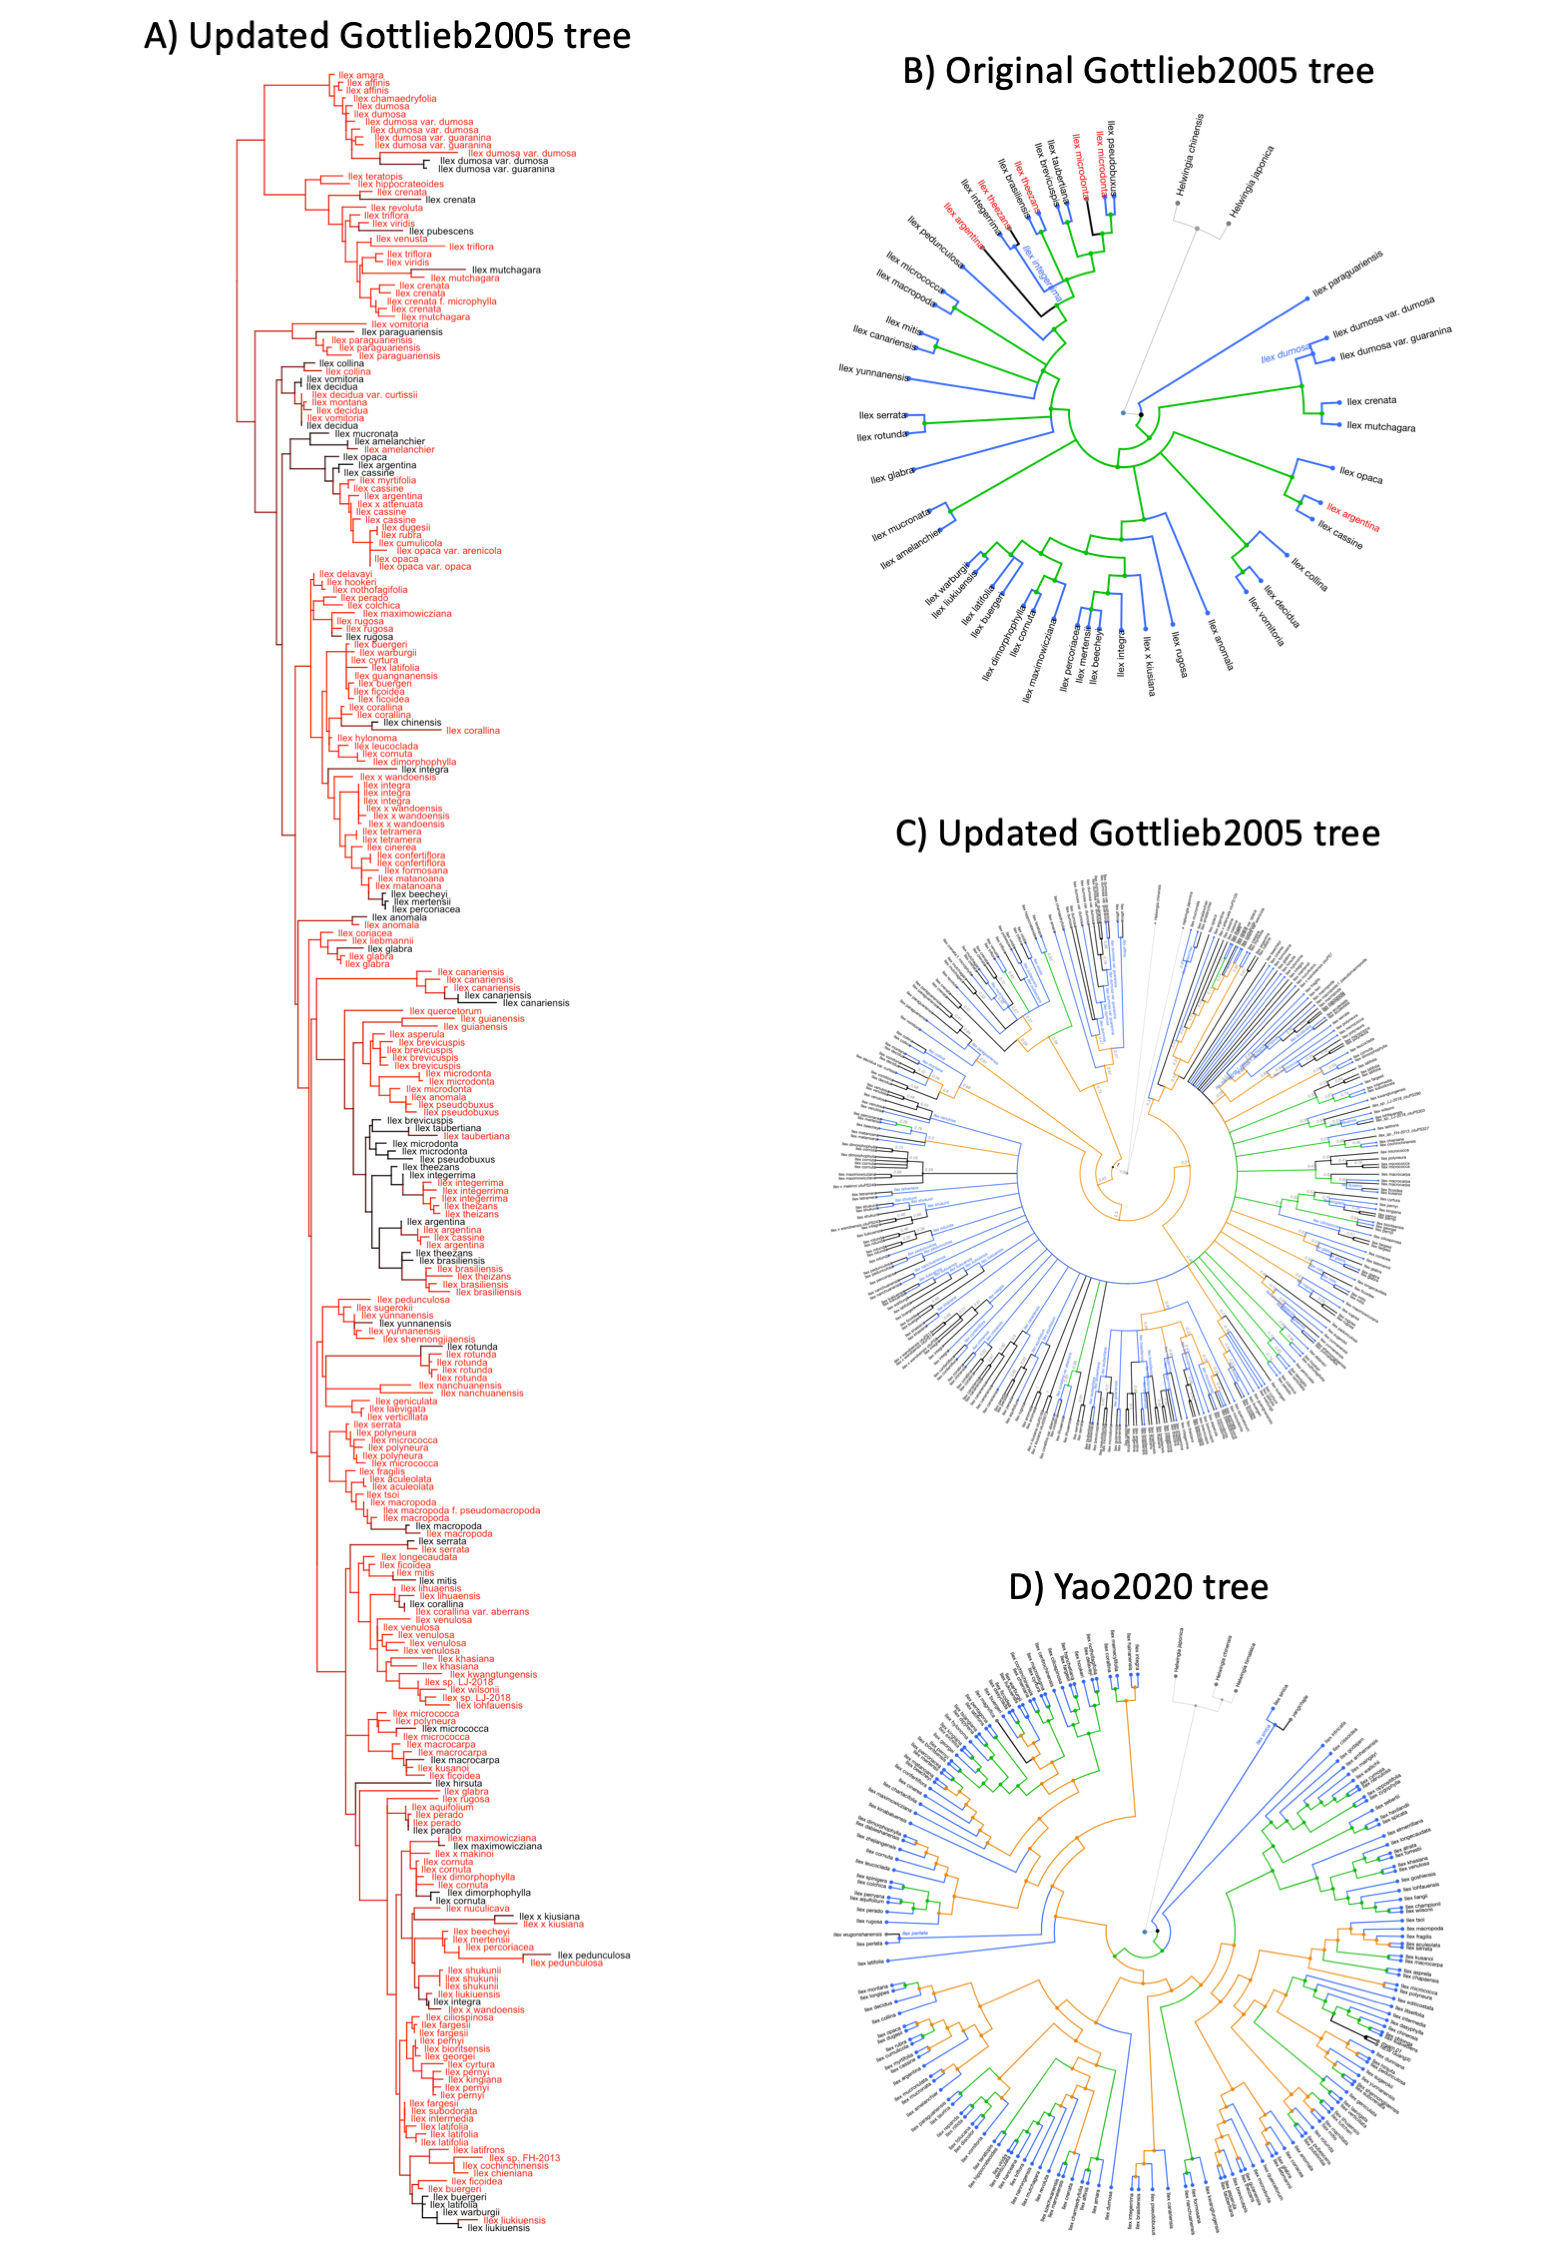
\includegraphics[width=1\linewidth]{docs/figs/ilex-results} \caption{A) Phylogenetic tree obtained by updating the Gottlieb et al. 2005 tree in B) using Physcraper.}\label{fig:results}
\end{figure}

\newpage

\emph{Figure \ref{fig:results} caption continued}: Tips in original alignment and new tips added with Physcraper are depicted in black and red, respectively. Physcraper obtained sequences from the GenBank database via local BLAST of all sequences in the original alignment that generated tree in B), filtered them following criteria specified in section ``DNA sequence search and filtering'', aligned them to the original alignment using MUSCLE and performed a phylogenetic reconstruction using RAxML with 100 bootstraps. B-D show results of the conflict analysis comparing estimated relationships to taxonomy, performed with OpenTree tools.

\hypertarget{discussion}{%
\section{Discussion}\label{discussion}}

Data repositories designed to preserve and democratize access to biological data
are essential resources for evolutionary estimation. While data keep accumulating,
our ability to reanalyze and incorporate new data with available knowledge is being challenged.

While phylogenetic pipelines designed to make evolutionary sense of the vast amount of public molecular data are available (e.g., Phylota (Sanderson \emph{et al.} \protect\hyperlink{ref-sanderson2008phylota}{2008}), PyPHLAWD (Smith \emph{et al.} \protect\hyperlink{ref-smith2009mega}{2009}), SUPERSMART (Antonelli \emph{et al.} \protect\hyperlink{ref-antonelli2017toward}{2017})), they focus on generating full trees \emph{de novo} (i.e., inferring phylogenetic relationships from a newly generated homology hypothesis, as opposed to e.g., supertrees, that are generated by assembling previous phylogenetic estimates).
While Physcraper does not generate phylogenies \emph{de novo} in a traditional sense,
it successfully generates new phylogenetic knowledge, revealing the potential of
phylogenetic knowledge published in databases to facilitate phylogenetic placement of public molecular data.
The PUMPER pipeline (Izquierdo-Carrasco \emph{et al.} \protect\hyperlink{ref-izquierdo2014pumper}{2014}) also uses the concept of updating
pre-existing alignments to incorporate public molecular data into phylogenies. Unfortunately, installation of the tool was unsuccesful following instructions from the author, and we were unable to benchmark a comparison.

Physcraper generates individual gene trees, which fail to capture the complexity of species' evolutionary history (Song \emph{et al.} \protect\hyperlink{ref-song2012resolving}{2012}). Yet, Physcraper makes it straightforward to gather alignments and gene trees for multiple loci from a taxonomic group of interest, which can then be used by any tool that performs coalescent analyses to generate species trees, e.g., ASTRAL (Mirarab \emph{et al.} \protect\hyperlink{ref-mirarab2014astral}{2014}), BEAST2 (Bouckaert \emph{et al.} \protect\hyperlink{ref-bouckaert2019beast}{2019}), SVD Quartets (Chifman \& Kubatko \protect\hyperlink{ref-chifman2014quartet}{2014})).

Physcraper not only links molecular and tree databases, it can also link phylogenies to various biological databases, such as GBIF, the Paleobiology Database, and others, by leveraging the integrated taxonomy from OpenTree (Rees \& Cranston \protect\hyperlink{ref-rees2017automated}{2017}).

Physcraper in conjuction with OpenTree can be used to rapidly (in a matter of hours)
address challenges overarching both fields of ecology and evolution, such as
placing newly discovered species phylogenetically (Webb \emph{et al.} \protect\hyperlink{ref-webb2010biodiversity}{2010}),
obtaining trees for ecophylogenetic studies (Helmus \& Ives \protect\hyperlink{ref-helmus2012phylogenetic}{2012}),
systematizing molecular (and other) databases, i.e., curating taxonomic assignations (San Mauro \& Agorreta \protect\hyperlink{ref-san2010molecular}{2010}),
and generating custom species trees for ecological and evolutionary downstream analyses (Stoltzfus \emph{et al.} \protect\hyperlink{ref-stoltzfus2013phylotastic}{2013}).

Data repositories hold more information than meets the eye.
Besides the main data, they are rich sources of metadata that can be leveraged for the advantage of all areas of biology as well as the advancement of scientific policy and applications.
Usually, initial ideas about the data are changed by new analyses.
Physcraper can provide context for these ideas by streamlining inferences integrating new data with existing knowledge.

\hypertarget{acknowledgements}{%
\section{Acknowledgements}\label{acknowledgements}}

Research was supported by the grant ``Sustaining the Open Tree of Life'', National Science Foundation ABI No.~1759838, and ABI No.~1759846.
Computer time was provided by the Multi-Environment Research Computer for Exploration and Discovery (MERCED) cluster from the University of California, Merced (UCM), supported by the NSF Grant No.~ACI-1429783.

We thank the members of the OpenTree development team and the ``short bar'' Science and Engineering Building 1, UCM, joint lab paper discussion group for valuable comments on this manuscript.

The authors have no conflict of interest to declare.

\hypertarget{authors-contributions}{%
\section{Authors' Contributions}\label{authors-contributions}}

LLSR wrote the manuscript, alignment code, documentation, performed analyses and developed examples; MK wrote code for ncbidataparser module, filtering of sequences per OTU and using offline blast searches, wrote documentation and tests; EJM conceived study, wrote most of the code, documentation and tests.
All authors contributed to the manuscript and gave final approval for publication.

\hypertarget{data-archiving}{%
\section{Data Archiving}\label{data-archiving}}

Physcraper source code available at \url{https://github.com/McTavishLab/physcraper}

Documentation available at \url{https://physcraper.readthedocs.io/en/latest/index.html}

Illustrated examples available at \url{https://github.com/McTavishLab/physcraperex}

This is a reproducible manuscript available at \url{https://github.com/McTavishLab/physcraper_ms}

\hypertarget{references}{%
\section*{References}\label{references}}
\addcontentsline{toc}{section}{References}

\hypertarget{refs}{}
\leavevmode\hypertarget{ref-altschul1990basic}{}%
Altschul, S.F., Gish, W., Miller, W., Myers, E.W. \& Lipman, D.J. (1990). Basic local alignment search tool. \emph{Journal of molecular biology}, \textbf{215}, 403--410.

\leavevmode\hypertarget{ref-andermann2020guide}{}%
Andermann, T., Torres Jiménez, M.F., Matos-Maraví, P., Batista, R., Blanco-Pastor, J.L., Gustafsson, A.L.S., Kistler, L., Liberal, I.M., Oxelman, B., Bacon, C.D. \& Antonelli, A. (2020). A Guide to Carrying Out a Phylogenomic Target Sequence Capture Project. \emph{Frontiers in Genetics}, \textbf{10}.

\leavevmode\hypertarget{ref-antonelli2017toward}{}%
Antonelli, A., Hettling, H., Condamine, F.L., Vos, K., Nilsson, R.H., Sanderson, M.J., Sauquet, H., Scharn, R., Silvestro, D., Töpel, M. \& others. (2017). Toward a self-updating platform for estimating rates of speciation and migration, ages, and relationships of taxa. \emph{Systematic Biology}, \textbf{66}, 152--166.

\leavevmode\hypertarget{ref-benson2000genbank}{}%
Benson, D.A., Karsch-Mizrachi, I., Lipman, D.J., Ostell, J., Rapp, B.A. \& Wheeler, D.L. (2000). GenBank. \emph{Nucleic acids research}, \textbf{28}, 15--18.

\leavevmode\hypertarget{ref-bouckaert2019beast}{}%
Bouckaert, R., Vaughan, T.G., Barido-Sottani, J., Duchêne, S., Fourment, M., Gavryushkina, A., Heled, J., Jones, G., Kühnert, D., Maio, N.D., Matschiner, M., Mendes, F.K., Müller, N.F., Ogilvie, H.A., Plessis, L. du, Popinga, A., Rambaut, A., Rasmussen, D., Siveroni, I., Suchard, M.A., Wu, C.-H., Xie, D., Zhang, C., Stadler, T. \& Drummond, A.J. (2019). BEAST 2.5: An advanced software platform for Bayesian evolutionary analysis. \emph{PLOS Computational Biology}, \textbf{15}, e1006650.

\leavevmode\hypertarget{ref-camacho2009blast}{}%
Camacho, C., George, C., Vahram, A., Ning, M., Jason, P., Kevin, B. \& Thomas, L. (2009). BLAST+: Architecture and applications. \emph{BMC bioinformatics}, \textbf{10}, 421.

\leavevmode\hypertarget{ref-castresana2000selection}{}%
Castresana, J. (2000). Selection of conserved blocks from multiple alignments for their use in phylogenetic analysis. \emph{Molecular biology and evolution}, \textbf{17}, 540--552.

\leavevmode\hypertarget{ref-chifman2014quartet}{}%
Chifman, J. \& Kubatko, L. (2014). Quartet Inference from SNP Data Under the Coalescent Model. \emph{Bioinformatics}, \textbf{30}, 3317--3324.

\leavevmode\hypertarget{ref-cock2009biopython}{}%
Cock, P.J., Antao, T., Chang, J.T., Chapman, B.A., Cox, C.J., Dalke, A., Friedberg, I., Hamelryck, T., Kauff, F., Wilczynski, B. \& others. (2009). Biopython: Freely available python tools for computational molecular biology and bioinformatics. \emph{Bioinformatics}, \textbf{25}, 1422--1423.

\leavevmode\hypertarget{ref-cuenoud2000molecular}{}%
Cuénoud, P., Martinez, M.A. del P., Loizeay, P.-A., Spichiger, R., Andrews, S. \& Manen, J.-F. (2000). Molecular phylogeny and biogeography of the genus Ilex L.(Aquifoliaceae). \emph{Annals of Botany}, \textbf{85}, 111--122.

\leavevmode\hypertarget{ref-edgar2004muscle}{}%
Edgar, R.C. (2004). MUSCLE: Multiple sequence alignment with high accuracy and high throughput. \emph{Nucleic acids research}, \textbf{32}, 1792--1797.

\leavevmode\hypertarget{ref-fragoso2017pilot}{}%
Fragoso-Martínez, I., Salazar, G.A., Martínez-Gordillo, M., Magallón, S., Sánchez-Reyes, L., Lemmon, E.M., Lemmon, A.R., Sazatornil, F. \& Mendoza, C.G. (2017). A pilot study applying the plant anchored hybrid enrichment method to new world sages (salvia subgenus calosphace; lamiaceae). \emph{Molecular Phylogenetics and Evolution}, \textbf{117}, 124--134.

\leavevmode\hypertarget{ref-gottlieb2005molecular}{}%
Gottlieb, A.M., Giberti, G.C. \& Poggio, L. (2005). Molecular analyses of the genus Ilex (Aquifoliaceae) in southern south america, evidence from aflp and its sequence data. \emph{American Journal of Botany}, \textbf{92}, 352--369.

\leavevmode\hypertarget{ref-helmus2012phylogenetic}{}%
Helmus, M.R. \& Ives, A.R. (2012). Phylogenetic diversity--area curves. \emph{Ecology}, \textbf{93}, S31--S43.

\leavevmode\hypertarget{ref-izquierdo2014pumper}{}%
Izquierdo-Carrasco, F., Cazes, J., Smith, S.A. \& Stamatakis, A. (2014). PUmPER: Phylogenies updated perpetually. \emph{Bioinformatics}, \textbf{30}, 1476--1477.

\leavevmode\hypertarget{ref-jones2016targeted}{}%
Jones, M.R. \& Good, J.M. (2016). TARGETED capture in evolutionary and ecological genomics. \emph{Molecular ecology}, \textbf{25}, 185--202.

\leavevmode\hypertarget{ref-manen2010history}{}%
Manen, J.-F., Barriera, G., Loizeau, P.-A. \& Naciri, Y. (2010). The history of extant Ilex species (Aquifoliaceae): Evidence of hybridization within a miocene radiation. \emph{Molecular Phylogenetics and Evolution}, \textbf{57}, 961--977.

\leavevmode\hypertarget{ref-mirarab2014astral}{}%
Mirarab, S., Reaz, R., Bayzid, M.S., Zimmermann, T., Swenson, M.S. \& Warnow, T. (2014). ASTRAL: Genome-scale coalescent-based species tree estimation. \emph{Bioinformatics}, \textbf{30}, i541--i548.

\leavevmode\hypertarget{ref-morrison2006multiple}{}%
Morrison, D.A. (2006). Multiple sequence alignment for phylogenetic purposes. \emph{Australian Systematic Botany}, \textbf{19}, 479--539.

\leavevmode\hypertarget{ref-piel2009treebase}{}%
Piel, W., Chan, L., Dominus, M., Ruan, J., Vos, R. \& Tannen, V. (2009). Treebase v. 2: A database of phylogenetic knowledge. E-biosphere.

\leavevmode\hypertarget{ref-redelings2017supertree}{}%
Redelings, B.D. \& Holder, M.T. (2017). A supertree pipeline for summarizing phylogenetic and taxonomic information for millions of species. \emph{PeerJ}, \textbf{5}, e3058.

\leavevmode\hypertarget{ref-rees2017automated}{}%
Rees, J.A. \& Cranston, K. (2017). Automated assembly of a reference taxonomy for phylogenetic data synthesis. \emph{Biodiversity Data Journal}.

\leavevmode\hypertarget{ref-sanderson2008phylota}{}%
Sanderson, M.J., Boss, D., Chen, D., Cranston, K.A. \& Wehe, A. (2008). The PhyLoTA Browser: Processing GenBank for Molecular Phylogenetics Research. \emph{Systematic Biology}, \textbf{57}, 335--346.

\leavevmode\hypertarget{ref-san2010molecular}{}%
San Mauro, D. \& Agorreta, A. (2010). Molecular systematics: A synthesis of the common methods and the state of knowledge. \emph{Cellular \& Molecular Biology Letters}, \textbf{15}, 311.

\leavevmode\hypertarget{ref-secretariat2017gbif}{}%
Secretariat, G. (2017). GBIF backbone taxonomy. \emph{Checklist Dataset {[}cited 2017 Nov 14{]}. doi}, \textbf{10}.

\leavevmode\hypertarget{ref-selbach2009new}{}%
Selbach-Schnadelbach, A., Cavalli, S.S., Manen, J.-F., Coelho, G.C. \& De Souza-Chies, T.T. (2009). New information for Ilex phylogenetics based on the plastid psbA-trnH intergenic spacer (Aquifoliaceae). \emph{Botanical Journal of the Linnean Society}, \textbf{159}, 182--193.

\leavevmode\hypertarget{ref-setoguchi2000intersectional}{}%
Setoguchi, H. \& Watanabe, I. (2000). Intersectional gene flow between insular endemics of ilex (aquifoliaceae) on the bonin islands and the ryukyu islands. \emph{American Journal of Botany}, \textbf{87}, 793--810.

\leavevmode\hypertarget{ref-smith2009mega}{}%
Smith, S.A., Beaulieu, J.M. \& Donoghue, M.J. (2009). Mega-phylogeny approach for comparative biology: An alternative to supertree and supermatrix approaches. \emph{BMC evolutionary biology}, \textbf{9}, 37.

\leavevmode\hypertarget{ref-song2012resolving}{}%
Song, S., Liu, L., Edwards, S.V. \& Wu, S. (2012). Resolving conflict in eutherian mammal phylogeny using phylogenomics and the multispecies coalescent model. \emph{Proceedings of the National Academy of Sciences}, \textbf{109}, 14942--14947.

\leavevmode\hypertarget{ref-stamatakis2014raxml}{}%
Stamatakis, A. (2014). RAxML version 8: A tool for phylogenetic analysis and post-analysis of large phylogenies. \emph{Bioinformatics}, \textbf{30}, 1312--1313.

\leavevmode\hypertarget{ref-stoltzfus2013phylotastic}{}%
Stoltzfus, A., Lapp, H., Matasci, N., Deus, H., Sidlauskas, B., Zmasek, C.M., Vaidya, G., Pontelli, E., Cranston, K., Vos, R. \& others. (2013). Phylotastic! Making tree-of-life knowledge accessible, reusable and convenient. \emph{BMC bioinformatics}, \textbf{14}, 158.

\leavevmode\hypertarget{ref-sukumaran2010dendropy}{}%
Sukumaran, J. \& Holder, M.T. (2010). DendroPy: A python library for phylogenetic computing. \emph{Bioinformatics}, \textbf{26}, 1569--1571.

\leavevmode\hypertarget{ref-vos2012nexml}{}%
Vos, R.A., Balhoff, J.P., Caravas, J.A., Holder, M.T., Lapp, H., Maddison, W.P., Midford, P.E., Priyam, A., Sukumaran, J., Xia, X. \& others. (2012). NeXML: Rich, extensible, and verifiable representation of comparative data and metadata. \emph{Systematic biology}, \textbf{61}, 675--689.

\leavevmode\hypertarget{ref-webb2010biodiversity}{}%
Webb, C.O., Slik, J.F. \& Triono, T. (2010). Biodiversity inventory and informatics in southeast asia. \emph{Biodiversity and Conservation}, \textbf{19}, 955--972.

\leavevmode\hypertarget{ref-wheeler2000database}{}%
Wheeler, D.L., Chappey, C., Lash, A.E., Leipe, D.D., Madden, T.L., Schuler, G.D., Tatusova, T.A. \& Rapp, B.A. (2000). Database resources of the national center for biotechnology information. \emph{Nucleic acids research}, \textbf{28}, 10--14.

\leavevmode\hypertarget{ref-yao2020phylogeny}{}%
Yao, X., Song, Y., Yang, J.-B., Tan, Y.-H. \& Corlett, R.T. (2020). Phylogeny and biogeography of the hollies (ilex l., aquifoliaceae). \emph{Journal of Systematics and Evolution}.

\end{document}
